

%
% This is an example LaTeX presentation for Dept. of Math. Sciences 
% (University of Oulu) using Beamer and new 2016 logos of OU
%
% Required images are distributed with this template
%
% This example file contains basic environment's and properties of
% Beamer. For more detailed information, see e.g. Beamer manual.
%
% Author: Tero Vedenjuoksu, Markus Harju (Math. Dept., Oulu Uni)
%
% Use pdflatex to compile the PDF-file

\documentclass{beamer} %Presentation version
\usepackage{tikz}
\usetikzlibrary{calc}
\usetikzlibrary{babel}
%\documentclass[handout]{beamer} % For paper version (read the note below).
%\usepackage[latin1]{inputenc}
\usepackage[utf8]{inputenc} % Windows, utf8 file, works in Mac OS X too
\usepackage[T1]{fontenc}
\usepackage[percent]{overpic}
\usepackage{pgfplots}
\pgfplotsset{compat=1.6}
\pgfplotsset{soldot/.style={color=blue,only marks,mark=*}} \pgfplotsset{holdot/.style={color=blue,fill=white,only marks,mark=*}}
\usepackage{xcolor}
\usepackage{ifthen}
\usepackage{mathtools}
\usepackage{listofitems} % for \readlist to create arrays
\tikzstyle{mynode}=[thick,draw=blue,fill=blue!20,circle,minimum size=22]
\newboolean{FIN}
\setboolean{FIN}{true} % true=Finnish slides, false=English slides

\usepackage{amsmath,algorithm,float,tabularx,amsfonts}
\usepackage{algpseudocode}
\usepackage{graphicx}
\makeatletter
\renewcommand{\ALG@name}{Algoritmi}
\newcommand{\multiline}[1]{%
    \begin{tabularx}{\dimexpr\linewidth-\ALG@thistlm}[t]{@{}X@{}}
        #1
    \end{tabularx}
}
\newcommand{\Input}[1]{\algrenewcommand{\alglinenumber}[1]{\textbf{Syöttö:} \ \setcounter{ALG@line}{\numexpr##1-1}} #1}
\newcommand{\Step}[1]{\algrenewcommand{\alglinenumber}[1]{Askel ##1: } #1}
\newcommand{\NoNumber}{\algrenewcommand{\alglinenumber}[1]{\setcounter{ALG@line}{\numexpr##1-1} \ \ \ \ \ \ \ \ \ \ }}
\newcommand{\Output}[1]{\algrenewcommand{\alglinenumber}[1]{\textbf{Ulostulo:}\setcounter{ALG@line}{\numexpr##1-1}} #1}

\newcommand{\lang}[2]{\ifthenelse{\boolean{FIN}}{#1}{#2}}
\DeclarePairedDelimiter\norm{\lVert}{\rVert}%

\usepackage{deptmath2016} % This has to be before the following!

% NOTE! NOTE! NOTE! NOTE! NOTE! NOTE! NOTE! NOTE! 
% NOTE! NOTE! NOTE! NOTE! NOTE! NOTE! NOTE! NOTE! 
%
% To remove footline, uncomment the following line (e.g. handout version)
%\setbeamertemplate{footline}{\vspace{8.65pt}}

\usepackage{amsthm}  

% Define all thm environments you need like this
\newtheorem{thm}{\lang{Lause}{Theorem}}
\newtheorem{lem}{\lang{Lemma}{Lemma}}
\newtheorem{cor}{\lang{Seuraus}{Corollary}}
\theoremstyle{definition}
\newtheorem{defn}{\lang{Määritelmä}{Definition}}


%%%%%%%%%%%%%%%%%%%%%%%%%%%%%%%%%%%%%%%%%%%%%%%%%%%%%
%%%%%       D E F I N I T I O N S    %%%%%%%%%%%%%%%%
\ifthenelse{\boolean{FIN}}{\usepackage[finnish]{babel}}{ }%finnish hyphenation
\setbeamersize{text margin left=1cm}
\setbeamersize{text margin right=1.2cm}
\usepackage{amsfonts}
%%%%%       * * * * * * * * * * *    %%%%%%%%%%%%%%%%
%%%%%%%%%%%%%%%%%%%%%%%%%%%%%%%%%%%%%%%%%%%%%%%%%%%%%



% NOTE! NOTE! NOTE! NOTE! NOTE! NOTE! NOTE! NOTE! 
% NOTE! NOTE! NOTE! NOTE! NOTE! NOTE! NOTE! NOTE! 
%
% Uncomment the following three (3) lines if you DON'T want a sidebar.
% Sidebar is NOT recommended for smaller presenation!
% \useoutertheme[right, height=0pt,width=2cm]{sidebar}
% \setbeamersize{text margin left=0.7cm}
% \setbeamersize{text margin right=0.5cm}


%%% main matter info, must be in premble to avoid a warning
\title{Myötäsyötteiset neuroverkot}
\author[Jimi Käyrä]{Jimi Käyrä}
\institute[Oulun yliopisto]{Oulun yliopisto}
\date[15.12.2022]{15.12.2022} 
%\usetikzlibrary{calc}

\begin{document}


%%% Making titlepage
\renewcommand{\headrulewidth}{0pt}  
\renewcommand{\footrulewidth}{0pt}

%\section{home}
\frame{\titlepage}
\setlength{\headheight}{0pt}

% Presentation structure
\section{Neuroverkon rakenne ja toiminta}
\section{Neuroverkon opettaminen}
    \subsection{Method 1}

\subsection{subsection title1}
\begin{frame}\frametitle{Ohjatun oppimisen malli}
\begin{itemize}
\item Mallia opetetaan opetusdatajoukolla \[L=\{(x^{(1)}, y^{(1)}), \ldots, (x^{(M)}, y^{(M)})\}\subset X\times Y,\] jossa \(x^{(i)}\in X\) on opetusesimerkin \(i\) piirrevektori ja \(y^{(i)}\in Y\) vastaava kohdemuuttujan arvo.

\item Tavoitteena on etsiä sellainen kuvaus \(g : X\to Y\), että \(g(x)\) vastaa mahdollisimman hyvin tuntematonta arvoa, kun \(x\in X\) on opetusdataan kuulumaton piirrevektori.

\end{itemize}\vspace{0.2in}

\begin{center}
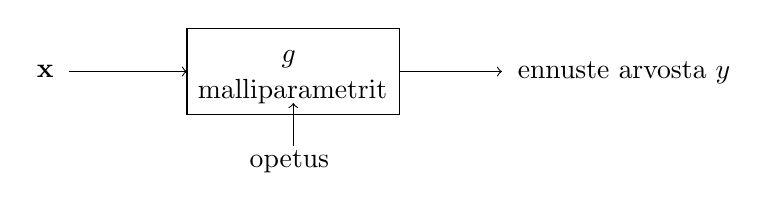
\begin{tikzpicture}
\node[] at (-1.8,0.75) {\(\textbf{x}\)};
\node[] at (5.55,0.74) {ennuste arvosta \(y\)};

\draw [-to](-1.5,0.75)--(0,0.75);
\draw [-to](2.7,0.75)--(4,0.75);

\filldraw[fill=none] (0,0.2) rectangle (2.7,1.3);
\draw [-to](1.35,-0.2)--(1.35,0.35);
\node[] at (1.3,-0.4) {opetus};

%\draw [-to](8.05,1.25)--(9.5,1.25);
\node[] at (1.29,0.9) {\(g\)};
\node[] at (1.34,0.5) {malliparametrit};
\end{tikzpicture}
\end{center}
\end{frame}

\begin{frame}[fragile]\frametitle{Opetuksen ongelmia}
\begin{center}
%\begin{figure}
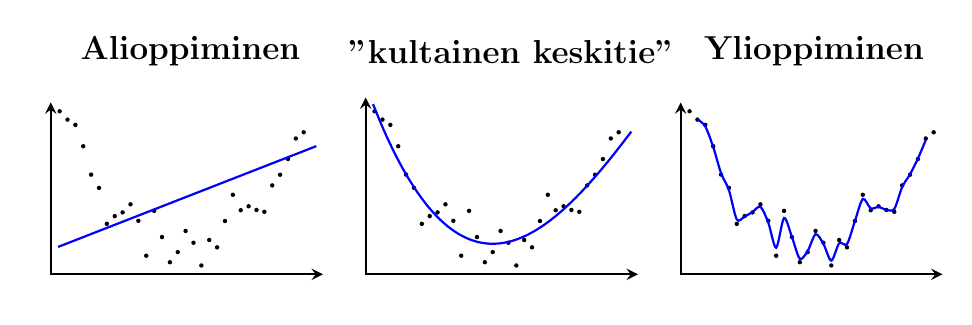
\begin{tikzpicture}[scale=0.8,declare function={f(\x)=0.5*pow(abs(\x-2),2)-0.06*pow(\x-2,3);}]
 \pgfmathsetseed{3333}
 \foreach \Z in {1,...,32}
 {\pgfmathsetmacro{\X}{\Z/8}
 \pgfmathsetmacro{\Y}{f(\X)+0.9*rnd}
 \ifnum\Z=1
  \xdef\LstOne{(\X,\Y)}
  \xdef\LstTwo{"(\X,\Y)"}
 \else
  \xdef\LstOne{\LstOne (\X,\Y)}
  \xdef\LstTwo{\LstTwo,"(\X,\Y)"}
 \fi}
 \begin{scope}[local bounding box=over,xshift=-5cm]
 \foreach \Z in {1,...,30}
 {\pgfmathsetmacro{\Last}{{\LstTwo}[\Z-1]}
 \pgfmathsetmacro{\Current}{{\LstTwo}[\Z]}
 \pgfmathsetmacro{\Next}{{\LstTwo}[\Z+1]}
  \edef\temp{\noexpand\path ($0.8*\Current+0.1*\Last+0.1*\Next$)   coordinate 
  (p\Z);}
  \temp
  \ifnum\Z=1
  \xdef\LstThree{(p\Z)}
  \else
  \xdef\LstThree{\LstThree (p\Z)}
  \fi
  }
 \foreach \Z in {1,...,32}
 {\pgfmathsetmacro{\Coor}{{\LstTwo}[\Z-1]}
 \fill \Coor circle[radius=1pt];
 }
 \draw[thick,blue] plot[smooth] coordinates \LstThree;
 \end{scope}
 %
 \begin{scope}[local bounding box=good,xshift=-10cm]
 \foreach \Z in {1,...,32}
 {\pgfmathsetmacro{\Coor}{{\LstTwo}[\Z-1]}
 \fill \Coor circle[radius=1pt];
 }
 \draw[thick,blue] plot[smooth,domain=0.1:4.2,variable=\x] (\x,{f(\x)+0.45});
 \end{scope}
 %
 \begin{scope}[local bounding box=under,xshift=-15cm]
 \foreach \Z in {1,...,32}
 {\pgfmathsetmacro{\Coor}{{\LstTwo}[\Z-1]}
 \fill \Coor circle[radius=1pt];
 }
 \draw[thick,blue] (0.1,0.4) -- (4.2,2);
 \end{scope}
 %
 \foreach \X in {over,good,under}
 {
 ([xshift=3pt,yshift=-3pt]\X.south east);
 \draw[stealth-stealth,thick] ([xshift=-3pt,yshift=3pt]\X.north west) node[left=5pt, below=40pt]{} 
 |- ([xshift=3pt,yshift=-3pt]\X.south east) node[left=65pt, below=1pt]{};}

 \node[] at (-12.8,3.5) {\large \textbf{Alioppiminen}};
  \node[] at (-7.7,3.5) {\large \textbf{"kultainen keskitie"}};
\node[] at (-2.9,3.5) {\large \textbf{Ylioppiminen}};
\end{tikzpicture}
%\end{figure}
\end{center}
\end{frame}

\begin{frame}\frametitle{Keinotekoinen neuroni}
\begin{center}
\includegraphics[scale=0.5]{bioneuron.png}
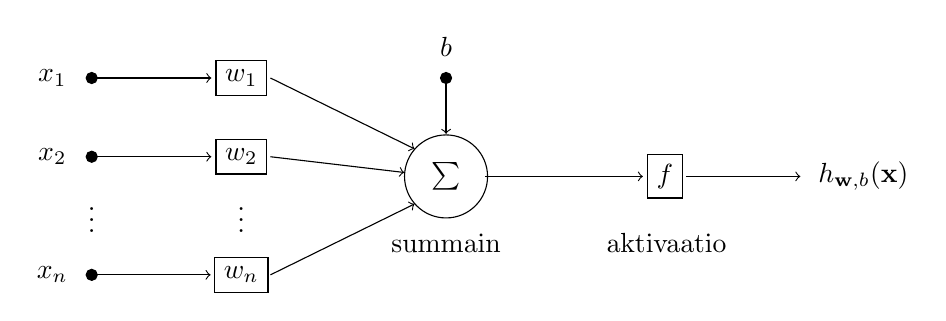
\begin{tikzpicture}
\node[] at (0,0) {\(x_n\)};
\draw [-to](0.5,0)--(2.01,0);
\filldraw (0.5,0) circle (2pt);
\node[draw] at (2.4,0) {\(w_n\)};

\node[] at (0,1.5) {\(x_2\)};
\draw [-to](0.5,1.5)--(2.02,1.5);
\filldraw (0.5,1.5) circle (2pt);
\node[draw] at (2.4,1.5) {\(w_2\)};

\node[] at (0,2.5) {\(x_1\)};
\draw [-to](0.5,2.5)--(2.02,2.5);
\filldraw (0.5,2.5) circle (2pt);
\node[draw] at (2.4,2.5) {\(w_1\)};

\node[] at (2.4,0.8) {\(\vdots\)};
\node[] at (0.5,0.8) {\(\vdots\)};

\draw (5,1.25) circle (15pt);
\draw [-to](5.5,1.25)--(7.5,1.25);
\node[draw] at (7.78,1.25) {\(f\)};
\node[] at (7.8,0.4) {aktivaatio};

\draw [-to](5,2.5)--(5,1.79);
\filldraw (5,2.5) circle (2pt);
\node[] at (5,2.9) {\(b\)};

\draw [-to](2.77,2.5)--(4.6,1.6);
\draw [-to](2.77,1.5)--(4.47,1.3);
\draw [-to](2.77,0)--(4.6,0.9);

\node[] at (5,1.25) {\(\sum\)};
\node[align=center] at (5,0.4) {summain};

\draw [-to](8.05,1.25)--(9.5,1.25);
\node[] at (10.3,1.25) {\(h_{\textbf{w},b}(\textbf{x})\)};
\end{tikzpicture}
\[h_{\textbf{w},b}(\mathbf{x})=f\left (b+\sum_{i=1}^{n} w_i x_i\right)=f(\textbf{w}^\top \textbf{x}+b)\]
\end{center}
\end{frame}

\begin{frame}\frametitle{Aktivaatiofunktio}
\begin{itemize}
\item Summaimen lähtö \(\textbf{w}^{\top}\textbf{x}+b\) on syötteen \(\textbf{x}\) affiini muunnos\\
\(\Rightarrow\) aktivaatiofunktio \(f\) mahdollistaa \alert{epälineaarisuuden}
\item Kynnystys (vrt. biologinen neuroni)
\end{itemize}
\vspace{0.2in}
\begin{center}
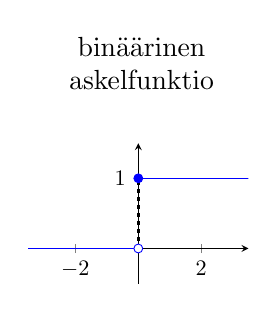
\begin{tikzpicture}[scale=0.8]
\node[align=center] at (1.8,3.5) {binäärinen\\askelfunktio};
\begin{axis}[height=1.5in,width=2in,axis x line=center,
  axis y line=center,
  xtick={-3,-4,...,3},
  ytick={0,1},
  xlabel={},
  ylabel={},
  xlabel style={right},
  ylabel style={above},
  xmin=-3.5,
  xmax=3.5,
  ymin=-0.5,
  ymax=1.5]
\addplot[domain=-5:0,blue] {0};
\addplot[domain=0:5,blue] {1};
%\addplot[domain=4:6,blue] {x};
%\addplot[domain=6:10,blue] {-5};
\draw[dotted,ultra thick] (axis cs:0,0) -- (axis cs:0,1);
\addplot[holdot] coordinates{(0,0)};
\addplot[soldot] coordinates{(0,1)};
\end{axis}
\end{tikzpicture}
\quad
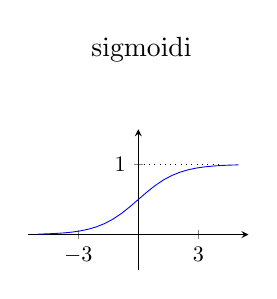
\begin{tikzpicture}[scale=0.8]
\node[align=center] at (1.8,3.5) {sigmoidi};
\begin{axis}[height=1.5in,width=2in,axis x line=center,
  axis y line=center,
  xtick={-3,3},
  ytick={0,1},
  xlabel={},
  ylabel={},
  xlabel style={right},
  ylabel style={above},
  xmin=-5.5,
  xmax=5.5,
  ymin=-0.5,
  ymax=1.5]
  
\addplot[domain=-5:5,blue] {1 / (1 + exp(-x))};
%\addplot[domain=4:6,blue] {x};
%\addplot[domain=6:10,blue] {-5};
\draw[dotted] (axis cs:0,1) -- (axis cs:4,1);
\end{axis}
\end{tikzpicture}
\quad
\begin{tikzpicture}[scale=0.8]
\node[align=center] at (1.8,3.5) {ReLU};
\begin{axis}[height=1.5in,width=2in,axis x line=center,
  axis y line=center,
  xtick={-2,2},
  ytick={0,1},
  xlabel=,
  ylabel={},
  xlabel style={right},
  ylabel style={above},
  xmin=-2.5,
  xmax=2.5,
  ymin=-0.5,
  ymax=1.5]
\addplot[domain=-5:0,blue] {0};
\addplot[domain=0:5,blue] {x};
%\addplot[domain=4:6,blue] {x};
%\addplot[domain=6:10,blue] {-5};
\addplot[soldot] coordinates{(0,0)};
\end{axis}
\end{tikzpicture}
\end{center}
\end{frame}

\begin{frame}\frametitle{Bias}
\begin{itemize}
\item Aktivaatioon vaadittavan kynnyksen säätö
\item Voidaan mieltää vakiosyötteeksi
\end{itemize}
\vspace{0.1in}
\begin{center}
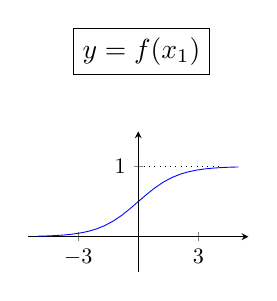
\begin{tikzpicture}[scale=0.8]
\node[draw] at (1.8,3.5) {\(y=f(x_1)\)};
\begin{axis}[height=1.5in,width=2in,axis x line=center,
  axis y line=center,
  xtick={-3,3},
  ytick={0,1},
  xlabel={},
  ylabel={},
  xlabel style={right},
  ylabel style={above},
  xmin=-5.5,
  xmax=5.5,
  ymin=-0.5,
  ymax=1.5]
  
\addplot[domain=-5:5,blue] {1 / (1 + exp(-x))};
%\addplot[domain=4:6,blue] {x};
%\addplot[domain=6:10,blue] {-5};
\draw[dotted] (axis cs:0,1) -- (axis cs:4,1);
\end{axis}
\end{tikzpicture}
\quad
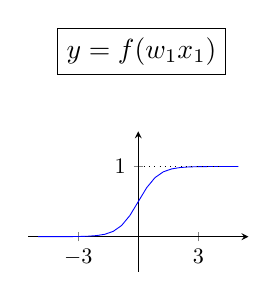
\begin{tikzpicture}[scale=0.8]
\node[draw] at (1.8,3.5) {\(y=f(w_1 x_1)\)};
\begin{axis}[height=1.5in,width=2in,axis x line=center,
  axis y line=center,
  xtick={-3,3},
  ytick={0,1},
  xlabel={},
  ylabel={},
  xlabel style={right},
  ylabel style={above},
  xmin=-5.5,
  xmax=5.5,
  ymin=-0.5,
  ymax=1.5]
  
\addplot[domain=-5:5,blue] {1 / (1 + exp(-(2*x)))};
%\addplot[domain=4:6,blue] {x};
%\addplot[domain=6:10,blue] {-5};
\draw[dotted] (axis cs:0,1) -- (axis cs:4,1);
\end{axis}
\end{tikzpicture}
\quad
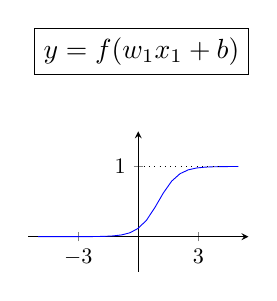
\begin{tikzpicture}[scale=0.8]
\node[draw] at (1.8,3.5) {\(y=f(w_1 x_1+b)\)};
\begin{axis}[height=1.5in,width=2in,axis x line=center,
  axis y line=center,
  xtick={-3,3},
  ytick={0,1},
  xlabel={},
  ylabel={},
  xlabel style={right},
  ylabel style={above},
  xmin=-5.5,
  xmax=5.5,
  ymin=-0.5,
  ymax=1.5]
  
\addplot[domain=-5:5,blue] {1 / (1 + exp(-(2*x-2)))};
%\addplot[domain=4:6,blue] {x};
%\addplot[domain=6:10,blue] {-5};
\draw[dotted] (axis cs:0,1) -- (axis cs:4,1);
\end{axis}
\end{tikzpicture}
\end{center}
\end{frame}

\begin{frame}\frametitle{Neuroverkon arkkitehtuuri}
\begin{defn}
Neuroverkon arkkitehtuuri voidaan kuvata järjestettynä nelikkona \((I, L, O, E)\), jossa \(I\) on syötepaikkojen joukko, \(L\) laskentayksikkösolmujen joukko, \(O\) lähtöpaikkojen joukko ja \(E\) joukko, joka koostuu painotetuista, suunnatuista linkeistä. Linkki on kolmikko \((u, v, w)\), jossa \(u\in I\cup L\), \(v\in L\cup O\) ja \(w\in \mathbb{R}\).
\end{defn}

\begin{defn}
Neuroverkko on myötäsyötteinen (\textit{feed-forward}) täsmälleen silloin, kun se ei sisällä syklejä.
\end{defn}
\end{frame}

\begin{frame}\frametitle{Neuroverkon arkkitehtuuri}
\begin{itemize}
    \item Merkitään
    \begin{itemize}
        \item \(w_{ij}^{(l)}\): kerroksen \(L_{l+1}\) neuronia \(i\) ja kerroksen \(L_l\) neuronia \(j\) yhdistävän linkin paino,
        \item \(b_i^{(l)}\): kerroksen \(L_{l+1}\) neuronin \(i\) bias-termi,
        \item \(h_i^{(l)}\): kerroksen \(L_l\) neuronin \(i\) lähtö.
    \end{itemize}
\end{itemize}
\begin{center}
\tikzset{%
  every neuron/.style={
    circle,
    draw,
    minimum size=1cm
  },
  neuron missing/.style={
    draw=none, 
    scale=3,
    text height=0.333cm,
    execute at begin node=\color{black}$\vdots$
  },
}

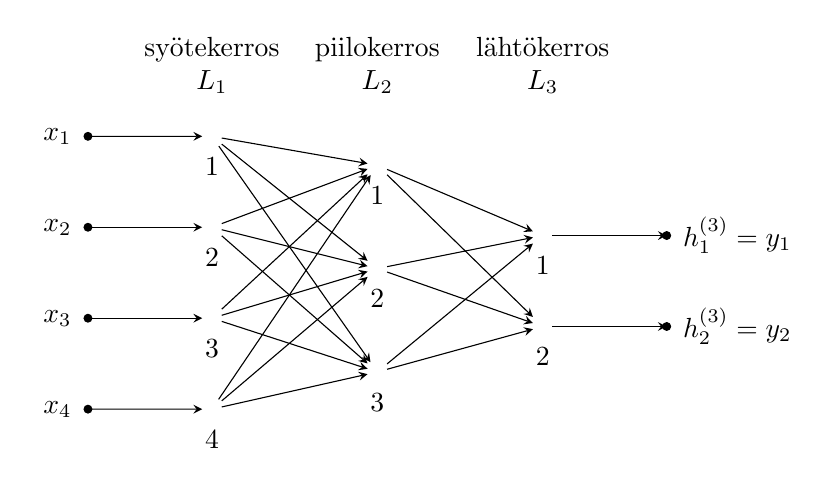
\begin{tikzpicture}[scale=0.7,x=1.5cm, y=1.5cm, >=stealth]

\foreach \m/\l [count=\y] in {1,2,3,4}
  \node [every neuron/.try, neuron \m/.try] (input-\m) at (0,2.5-\y*1.1) {};

\foreach \m [count=\y] in {1,2,3}
  \node [every neuron/.try, neuron \m/.try] (hidden-\m) at (2,2.3-\y*1.25) {};

\foreach \m [count=\y] in {1,2}
  \node [every neuron/.try, neuron \m/.try ] (output-\m) at (4,1.3-\y*1.1) {};

\foreach \l [count=\i] in {1,2,3,4}
  \draw [<-] (input-\i) -- ++(-1.5,0)
    node [left,inner sep=0.2cm] {$x_\l$};
  %\node[] at (0,1.5) {\(x_2\)};
  
\foreach \l [count=\i] in {1,2,3,4}
  \filldraw (input-\i)++(-1.5,0) circle (2pt);
    
\foreach \l [count=\i] in {1,2,3,4} % syötekerroksen numerot
  \node [shift={(0,-0.34)}] at (input-\i.north) {\l};

\foreach \l [count=\i] in {1,2,3} % piilokerroksen numerot
  \node [shift={(0,-0.34)}] at (hidden-\i.north) {\l};
  
\foreach \l [count=\i] in {1,2} % lähtökerroksen numerot
  \node [shift={(0,-0.34)}] at (output-\i.north) {\l};

\foreach \l [count=\i] in {1,2}
  \draw [->] (output-\i) -- ++(1.5,0)
    node [right,inner sep=0.2cm] {$h_\l^{(3)}=y_\l$};


\foreach \l [count=\i] in {1,2}
    \filldraw (output-\i)++(1.5,0) circle (2pt);

\foreach \i in {1,...,4}
  \foreach \j in {1,...,3}
    \draw [->] (input-\i) -- (hidden-\j);

\foreach \i in {1,...,3}
  \foreach \j in {1,...,2}
    \draw [->] (hidden-\i) -- (output-\j);

\foreach \l [count=\x from 0] in {syötekerros\\ \(L_1\), piilokerros\\ \(L_2\), lähtökerros\\ \(L_3\)}
\node [align=center, above] at (\x*2,1.8) {\l};

\end{tikzpicture}
\end{center}
\end{frame}

\begin{frame}\frametitle{Myötäsyöttöprosessi}
\begin{itemize}
    \item Miten määrätään verkon lähtö (output), kun syöte (input) tunnetaan?
    
    \item Käytetään syötekerroksen neuronien lähtöjä seuraavan kerroksen neuronien syötteinä ja lasketaan neuronien lähtö.
    
    \item Edetään näin rekursiivisesti lähtökerrokseen asti.
\end{itemize}
\end{frame}

\begin{frame}\frametitle{Myötäsyöttöprosessi}
\[\textcolor{blue}{h^{(1)}}=\textcolor{red}{\textbf{x}}=\textcolor{red}{(x_1, x_2, x_3, x_4)}\]
\begin{center}
\tikzset{%
  every neuron/.style={
    circle,
    draw,
    minimum size=1cm
  },
  neuron missing/.style={
    draw=none, 
    scale=3,
    text height=0.333cm,
    execute at begin node=\color{black}$\vdots$
  },
}

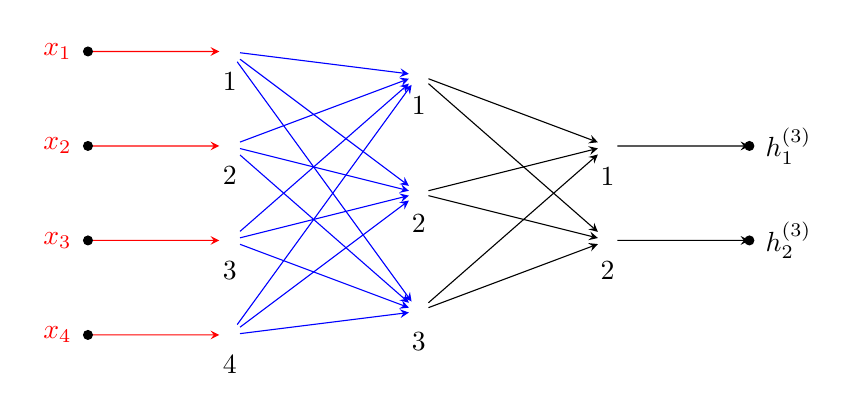
\begin{tikzpicture}[scale=0.8,x=1.5cm, y=1.5cm, >=stealth]


\foreach \m/\l [count=\y] in {1,2,3,4}
  \node [every neuron/.try, neuron \m/.try,thick] (input-\m) at (0,2.5-\y) {};

\foreach \m [count=\y] in {1,2,3}
  \node [every neuron/.try, neuron \m/.try] (hidden-\m) at (2,2.5-\y*1.25) {};

\foreach \m [count=\y] in {1,2}
  \node [every neuron/.try, neuron \m/.try ] (output-\m) at (4,1.5-\y) {};

\foreach \l [count=\i] in {1,2,3,4}
  \draw [<-,red] (input-\i) -- ++(-1.5,0)
    node [left,inner sep=0.2cm, red] {$x_\l$};
  %\node[] at (0,1.5) {\(x_2\)};
  
\foreach \l [count=\i] in {1,2,3,4}
  \filldraw (input-\i)++(-1.5,0) circle (2pt);
    
\foreach \l [count=\i] in {1,2,3,4} % syötekerroksen numerot
  \node [shift={(0,-0.34)}] at (input-\i.north) {\l};

\foreach \l [count=\i] in {1,2,3} % piilokerroksen numerot
  \node [shift={(0,-0.34)}] at (hidden-\i.north) {\l};
  
\foreach \l [count=\i] in {1,2} % lähtökerroksen numerot
  \node [shift={(0,-0.34)}] at (output-\i.north) {\l};

\foreach \l [count=\i] in {1,2}
  \draw [->] (output-\i) -- ++(1.5,0)
    node [right,inner sep=0.2cm] {$h_\l^{(3)}$};


\foreach \l [count=\i] in {1,2}
    \filldraw (output-\i)++(1.5,0) circle (2pt);

\foreach \i in {1,...,4}
  \foreach \j in {1,...,3}
    \draw [->,blue] (input-\i) -- (hidden-\j);

\foreach \i in {1,...,3}
  \foreach \j in {1,...,2}
    \draw [->] (hidden-\i) -- (output-\j);

%\foreach \l [count=\x from 0] in {syötekerros\\ %\(L_1\), piilokerros\\ \(L_2\), lähtökerros\\ \(L_3\)}
%\node [align=center, above] at (\x*2,2) {\l};

\end{tikzpicture}
\end{center}
\end{frame}

\begin{frame}\frametitle{Myötäsyöttöprosessi}
\[\textcolor{blue}{h^{(2)}}=f(z^{(2)})=f(W^{(1)}\textcolor{red}{h^{(1)}}+b^{(1)})\]
\begin{center}
\tikzset{%
  every neuron/.style={
    circle,
    draw,
    minimum size=1cm
  },
  neuron missing/.style={
    draw=none, 
    scale=3,
    text height=0.333cm,
    execute at begin node=\color{black}$\vdots$
  },
}

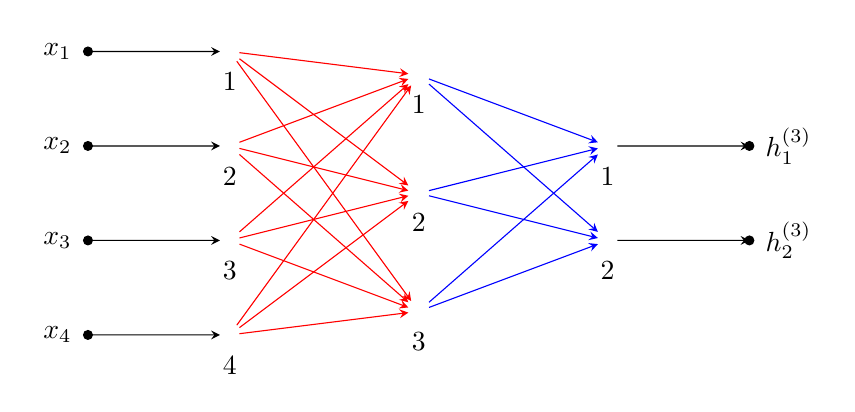
\begin{tikzpicture}[scale=0.8,x=1.5cm, y=1.5cm, >=stealth]


\foreach \m/\l [count=\y] in {1,2,3,4}
  \node [every neuron/.try, neuron \m/.try] (input-\m) at (0,2.5-\y) {};

\foreach \m [count=\y] in {1,2,3}
  \node [every neuron/.try, neuron \m/.try,thick] (hidden-\m) at (2,2.5-\y*1.25) {};

\foreach \m [count=\y] in {1,2}
  \node [every neuron/.try, neuron \m/.try ] (output-\m) at (4,1.5-\y) {};

\foreach \l [count=\i] in {1,2,3,4}
  \draw [<-] (input-\i) -- ++(-1.5,0)
    node [left,inner sep=0.2cm] {$x_\l$};
  %\node[] at (0,1.5) {\(x_2\)};
  
\foreach \l [count=\i] in {1,2,3,4}
  \filldraw (input-\i)++(-1.5,0) circle (2pt);
    
\foreach \l [count=\i] in {1,2,3,4} % syötekerroksen numerot
  \node [shift={(0,-0.34)}] at (input-\i.north) {\l};

\foreach \l [count=\i] in {1,2,3} % piilokerroksen numerot
  \node [shift={(0,-0.34)}] at (hidden-\i.north) {\l};
  
\foreach \l [count=\i] in {1,2} % lähtökerroksen numerot
  \node [shift={(0,-0.34)}] at (output-\i.north) {\l};

\foreach \l [count=\i] in {1,2}
  \draw [->] (output-\i) -- ++(1.5,0)
    node [right,inner sep=0.2cm] {$h_\l^{(3)}$};


\foreach \l [count=\i] in {1,2}
    \filldraw (output-\i)++(1.5,0) circle (2pt);

\foreach \i in {1,...,4}
  \foreach \j in {1,...,3}
    \draw [->,red] (input-\i) -- (hidden-\j);

\foreach \i in {1,...,3}
  \foreach \j in {1,...,2}
    \draw [->,blue] (hidden-\i) -- (output-\j);

%\foreach \l [count=\x from 0] in {syötekerros\\ %\(L_1\), piilokerros\\ \(L_2\), lähtökerros\\ \(L_3\)}
%\node [align=center, above] at (\x*2,2) {\l};

\end{tikzpicture}
\end{center}
\end{frame}

\begin{frame}\frametitle{Myötäsyöttöprosessi}
\[\textcolor{blue}{h^{(3)}}=f(z^{(3)})=f(W^{(2)}\textcolor{red}{h^{(2)}}+b^{(2)})\]
\begin{center}
\tikzset{%
  every neuron/.style={
    circle,
    draw,
    minimum size=1cm
  },
  neuron missing/.style={
    draw=none, 
    scale=3,
    text height=0.333cm,
    execute at begin node=\color{black}$\vdots$
  },
}

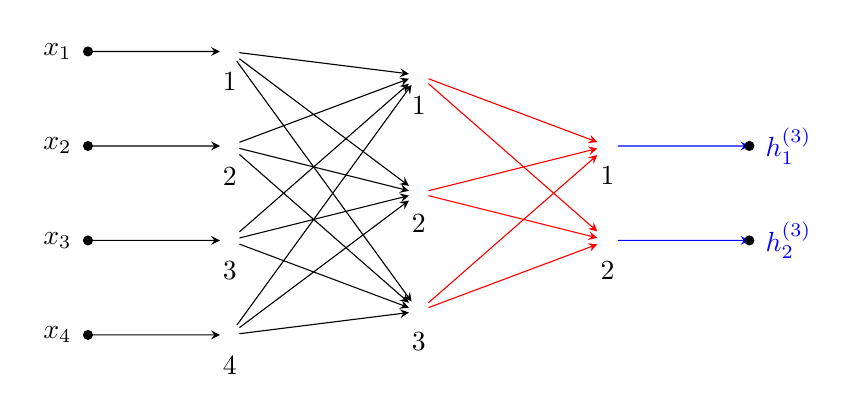
\begin{tikzpicture}[scale=0.8,x=1.5cm, y=1.5cm, >=stealth]


\foreach \m/\l [count=\y] in {1,2,3,4}
  \node [every neuron/.try, neuron \m/.try] (input-\m) at (0,2.5-\y) {};

\foreach \m [count=\y] in {1,2,3}
  \node [every neuron/.try, neuron \m/.try] (hidden-\m) at (2,2.5-\y*1.25) {};

\foreach \m [count=\y] in {1,2}
  \node [every neuron/.try, neuron \m/.try,thick] (output-\m) at (4,1.5-\y) {};

\foreach \l [count=\i] in {1,2,3,4}
  \draw [<-] (input-\i) -- ++(-1.5,0)
    node [left,inner sep=0.2cm] {$x_\l$};
  %\node[] at (0,1.5) {\(x_2\)};
  
\foreach \l [count=\i] in {1,2,3,4}
  \filldraw (input-\i)++(-1.5,0) circle (2pt);
    
\foreach \l [count=\i] in {1,2,3,4} % syötekerroksen numerot
  \node [shift={(0,-0.34)}] at (input-\i.north) {\l};

\foreach \l [count=\i] in {1,2,3} % piilokerroksen numerot
  \node [shift={(0,-0.34)}] at (hidden-\i.north) {\l};
  
\foreach \l [count=\i] in {1,2} % lähtökerroksen numerot
  \node [shift={(0,-0.34)}] at (output-\i.north) {\l};

\foreach \l [count=\i] in {1,2}
  \draw [->,blue] (output-\i) -- ++(1.5,0)
    node [right,inner sep=0.2cm] {$h_\l^{(3)}$};


\foreach \l [count=\i] in {1,2}
    \filldraw (output-\i)++(1.5,0) circle (2pt);

\foreach \i in {1,...,4}
  \foreach \j in {1,...,3}
    \draw [->] (input-\i) -- (hidden-\j);

\foreach \i in {1,...,3}
  \foreach \j in {1,...,2}
    \draw [->,red] (hidden-\i) -- (output-\j);

%\foreach \l [count=\x from 0] in {syötekerros\\ %\(L_1\), piilokerros\\ \(L_2\), lähtökerros\\ \(L_3\)}
%\node [align=center, above] at (\x*2,2) {\l};

\end{tikzpicture}
\end{center}
\end{frame}
% -pyrkii jäljittelemään hermoston toimintaa
% -perusyksikkönä neuroni
% koneoppiminen:
% menetelmien jaottelua: ohjattu/ohjaamaton/vahvistus\\
% sovelluskohteita\\
 %-> käytännössä kyse mallin sovittamisesta! => %optimointiformulointi
% haasteita, historiaa\\
 %ohjatun oppimisen malli kaaviona yleisellä tasolla: %syöte -> output, katsotaan miten hyvin vastaa tavoitetta %(virhefunktio) -> parametrien päivitys -> iteroidaan\\
 
 %neuroverkon biologinen inspiraatio ja vastaavuus\\
 %gradientti + laskeutuminen\\
 %Hadamard-tulo\\
%Any text or math...

\begin{frame}{}{size: 7pt}\frametitle{Neuroverkon opettaminen}
\begin{itemize}
    \item Miten määrätään opetusdatan avulla painot ja bias-termit siten, että verkko approksimoisi mahdollisimman hyvin syötteiden ja lähtöjen välistä riippuvuutta?
    
    \item Kvantifioidaan tavoite määrittelemällä aluksi yksittäiselle opetusesimerkille \((x^{(i)}, y^{(i)})\) virhefunktio
    \[\displaystyle J(W, b; x^{(i)}, y^{(i)})= \frac{1}{2}\norm{h_{W, b}(x^{(i)})-y^{(i)}}^2\]
    \begin{itemize}
        \item kuvaa verkon tuottaman ennusteen ja todellisen arvon välistä eroa
    \end{itemize}
\end{itemize}
\end{frame}

\begin{frame}{}{size: 7pt}\frametitle{Neuroverkon opettaminen}
\begin{itemize}
    \item Huomioidaan kaikki opetusnäytteet määrittelemällä kokonaisvirhefunktio
    \[ \scalebox{.9}{$\displaystyle J(W, b)=\underbrace{\frac{1}{M}\sum_{i=1}^{M} J(W, b; x^{(i)}, y^{(i)})}_{\text{keskineliövirhe}}+\underbrace{\frac{\lambda}{2}\sum_{l=1}^{n_l-1}\sum_{i=1}^{s_l}\sum_{j=1}^{s_{l+1}} \left(w_{ji}^{(l)}\right)^2}_{\text{painotermi}}$}.\]

    \item Tavoitteena on etsiä sellaiset \(W^*\) ja \(b^*\), että \(J\) minimoituu, ts. \[W^*, b^*=\text{arg min } J(W, b)\]
    \(\Rightarrow\) \alert{optimointiongelma}!
\end{itemize}
\end{frame}

\begin{frame}\frametitle{Gradienttilaskeutuminen}
\tikzset{>=latex}
\begin{center}
\begin{itemize}
\item Päivityssäännöt painoille ja biaksille:
\[w_{ij}^{(l)}\leftarrow w_{ij}^{(l)}-\alpha \frac{\partial J(W, b)}{\partial w_{ij}^{(l)}},\]
\[b_i^{(l)}\leftarrow b_i^{(l)}-\alpha \frac{\partial J(W, b)}{\partial b_i^{(l)}}.\]
\end{itemize}
    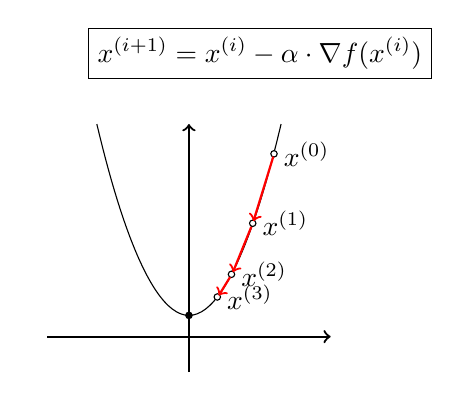
\begin{tikzpicture}[scale=0.9]
    \node[draw] at (1,4) {\(x^{(i+1)}=x^{(i)}-\alpha\cdot \nabla f(x^{(i)})\)};
    \draw[->=stealth, thick] (0,0)--(2,0) node[right]            {};
    \draw[thick] (0,0)--(-2,0) node[left] {};
    \draw[->=stealth, thick] (0,-0.5)--(0,3) node[above]{};

    \draw (0,0.3) parabola (1.3,3);
    \draw (0,0.3) parabola (-1.3,3);
    \draw[black,fill=black] (0,0.3) circle (.3ex);
    
    \draw[black,fill=white] (1.2,2.58) circle (.3ex) node[right] {\(x^{(0)}\)};
    \draw[black,fill=white] (0.9,1.6) circle (.3ex) node[right] {\(x^{(1)}\)};
    \draw[black,fill=white] (0.6,0.88) circle (.3ex) node[right] {\(x^{(2)}\)};
    \draw[black,fill=white] (0.4,0.56) circle (.3ex) node[right] {\(x^{(3)}\)};
    
    \draw[->=stealth,red,thick] (1.19,2.54)--(0.91,1.63);
    \draw[->=stealth,red,thick] (0.88,1.55)--(0.62,0.91);
    \draw[->=stealth,red,thick] (0.58,0.84)--(0.42,0.58);
    
    \end{tikzpicture}\hspace{0.2in}
    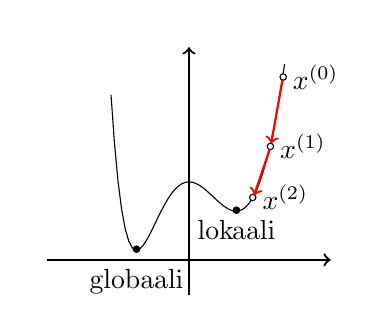
\begin{tikzpicture}[xscale=1,yscale=1,domain=-1.1:1.35,samples=50,scale=0.9]
    \draw[->=stealth, thick] (0,0)--(2,0) node[right]            {};
    \draw[thick] (0,0)--(-2,0) node[left] {};
    \draw[->=stealth, thick] (0,-0.5)--(0,3) node[above]{};
    
    \draw[black] plot (\x,{1.1+2.5*(-\x-1)*(-\x+1)*\x*\x*exp(-0.6*\x)});
    
    \draw[black,fill=white] (1.33,2.58) circle (.3ex) node[right] {\(x^{(0)}\)};
    \draw[black,fill=white] (1.15,1.6) circle (.3ex) node[right] {\(x^{(1)}\)};
    \draw[black,fill=white] (0.9,0.88) circle (.3ex) node[right] {\(x^{(2)}\)};
    
    \draw[->=stealth,red,thick] (1.32,2.54)--(1.16,1.64);
    \draw[->=stealth,red,thick] (1.14,1.56)--(0.92,0.91);
    
        \draw[black,fill=black] (0.67,0.7) circle (.3ex) node[below] {lokaali};

    \draw[black,fill=black] (-0.74,0.15) circle (.3ex) node[below=0.05in] {globaali};
    
    \end{tikzpicture}
\end{center}
\end{frame}

\begin{frame}{}{size: 7pt}\frametitle{Gradienttilaskeutuminen}
\begin{itemize}
    \item Suoralla laskulla havaitaan, että \begin{align*}
    &\frac{\partial J(W, b)}{\partial w_{ij}^{(l)}}=\frac{1}{M} \sum_{k=1}^{M} \textcolor{red}{\frac{\partial J(W, b; x^{(k)}, y^{(k)})}{\partial w_{ij}^{(l)}}}+\lambda w_{ij}^{(l)},\\
    &\frac{\partial J(W, b)}{\partial b_{i}^{(l)}}=\frac{1}{M} \sum_{k=1}^{M} \textcolor{blue}{\frac{\partial J(W, b; x^{(k)}, y^{(k)})}{\partial b_{i}^{(l)}}}.
\end{align*}
    
    \item Miten määrätään osittaisderivaatat \[\textcolor{red}{\frac{\partial J(W, b; x^{(i)}, y^{(i)})}{\partial w_{ij}^{(l)}}}\text{ ja }\textcolor{blue}{\frac{\partial J(W, b; x^{(i)}, y^{(i)})}{\partial b_{i}^{(l)}}}?\]
\end{itemize}
\end{frame}

\begin{frame}\frametitle{Vastavirta-algoritmi}
\begin{itemize}
\item Tarkastellaan ensin lähtökerrosta. Voidaan osoittaa, että nyt \[\frac{\partial J}{\partial w_{12}^{(2)}}=\frac{\partial J}{\partial h_1^{(3)}} \frac{\partial h_1^{(3)}}{\partial z_1^{(3)}} \frac{\partial z_1^{(3)}}{\partial w_{12}^{(2)}}=\underbrace{\left[-(y_1-h_1^{(3)})\cdot f'(z_1^{(3)})\right]}_{\textcolor{red}{\delta_1^{(3)}}}\textcolor{blue}{h_2^{(2)}}.\]

\item Yleisesti vektorimuodossa lähtökerrokselle \[\textcolor{red}{\delta^{(n_l)}}=-(y^{(i)}-h^{(n_l)})\odot f'(z^{(n_l)}),\] jolloin \[\frac{\partial J}{\partial W^{(n_l-1)}}=\textcolor{red}{\delta^{(n_l)}} (\textcolor{blue}{h^{(n_l-1)}})^{\top}.\]
\end{itemize}




\end{frame}

\begin{frame}\frametitle{Vastavirta-algoritmi}
\begin{itemize}
\item Havaitaan, että \textcolor{red}{piilokerroksen neuroni} vaikuttaa koko verkon lähtöön \textcolor{blue}{lähtökerroksen neuronien} välityksellä.
\end{itemize}
\begin{center}
\tikzset{%
  every neuron/.style={
    circle,
    draw,
    minimum size=1cm
  },
  neuron missing/.style={
    draw=none, 
    scale=3,
    text height=0.333cm,
    execute at begin node=\color{black}$\vdots$
  },
}

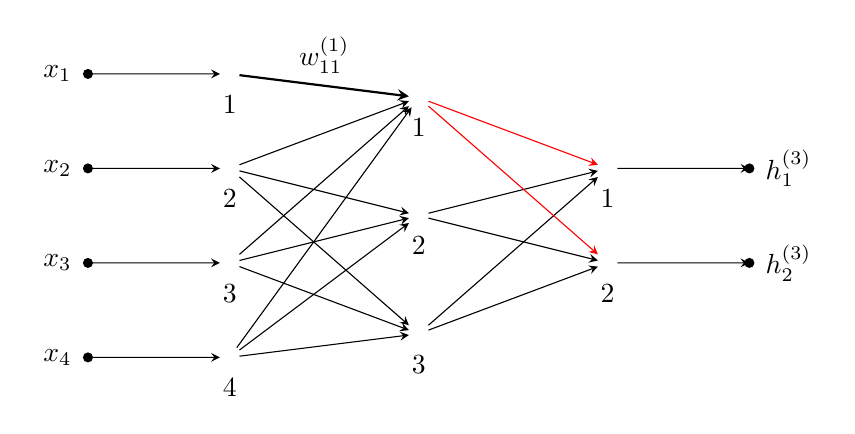
\begin{tikzpicture}[scale=0.8,x=1.5cm, y=1.5cm, >=stealth]
\node[] at (1.0,1.7) {\(w_{11}^{(1)}\)};

\foreach \m/\l [count=\y] in {1,2,3,4}
  \node [every neuron/.try, neuron \m/.try] (input-\m) at (0,2.5-\y) {};

\foreach \m [count=\y] in {2,3}
  \node [every neuron/.try, neuron \m/.try] (hidden-\m) at (2,1.25-\y*1.25) {};
\node [every neuron/.try, neuron 1/.try,red] (hidden-1) at (2,2.5-1*1.25) {};
  
\foreach \m [count=\y] in {1,2}
  \node [every neuron/.try, neuron \m/.try,blue ] (output-\m) at (4,1.5-\y) {};

\foreach \l [count=\i] in {1,2,3,4}
  \draw [<-] (input-\i) -- ++(-1.5,0)
    node [left,inner sep=0.2cm] {$x_\l$};
  %\node[] at (0,1.5) {\(x_2\)};
  
\foreach \l [count=\i] in {1,2,3,4}
  \filldraw (input-\i)++(-1.5,0) circle (2pt);
    
\foreach \l [count=\i] in {1,2,3,4} % syötekerroksen numerot
  \node [shift={(0,-0.34)}] at (input-\i.north) {\l};

\foreach \l [count=\i] in {1,2,3} % piilokerroksen numerot
  \node [shift={(0,-0.34)}] at (hidden-\i.north) {\l};
  
\foreach \l [count=\i] in {1,2} % lähtökerroksen numerot
  \node [shift={(0,-0.34)}] at (output-\i.north) {\l};

\foreach \l [count=\i] in {1,2}
  \draw [->] (output-\i) -- ++(1.5,0)
    node [right,inner sep=0.2cm] {$h_\l^{(3)}$};


\foreach \l [count=\i] in {1,2}
    \filldraw (output-\i)++(1.5,0) circle (2pt);

\foreach \i in {2,...,4}
  \foreach \j in {1,...,3}
    \draw [->] (input-\i) -- (hidden-\j);
\draw [->,thick] (input-1) -- (hidden-1);

\foreach \i in {2,...,3}
  \foreach \j in {1,...,2}
    \draw [->] (hidden-\i) -- (output-\j);
\draw [->,red] (hidden-1) -- (output-1);
\draw [->,red] (hidden-1) -- (output-2);

%\foreach \l [count=\x from 0] in {syötekerros\\ %\(L_1\), piilokerros\\ \(L_2\), lähtökerros\\ \(L_3\)}
%\node [align=center, above] at (\x*2,2) {\l};

\end{tikzpicture}
\end{center}
\end{frame}

\begin{frame}\frametitle{Vastavirta-algoritmi}
\begin{itemize}
\item Edetään piilokerrokseen kirjoittamalla \[\frac{\partial J}{\partial w_{11}^{(1)}}=\frac{\partial J}{\partial z_1^{(2)}}\frac{\partial z_1^{(2)}}{\partial w_{11}^{(1)}}=\left(\sum_{i=1}^{2} \underbrace{\frac{\partial J}{\partial z_i^{(3)}}}_{\textcolor{red}{\delta_i^{(3)}}}\frac{\partial z_i^{(3)}}{\partial z_1^{(2)}}\right)\frac{\partial z_1^{(2)}}{\partial w_{11}^{(1)}}\]
\\ \(\Rightarrow\) laskennassa voidaan hyödyntää \alert{edeltävän kerroksen}\\\hspace{0.2in}jo laskettuja virhetermejä!

\item Voidaan näyttää, että yleisesti piilokerroksille \[\delta^{(l)}=\left[(W^{(l)})^{\top} \textcolor{red}{\delta^{(l+1)}}\right]\odot f'(z^{(l)}),\] jolloin \[\frac{\partial J}{\partial W^{(l)}}=\delta^{(l+1)}(h^{(l)})^{\top}.\]

\end{itemize}
\end{frame}

\begin{frame}\frametitle{Vastavirta-algoritmi}
\begin{enumerate}
    \item Lasketaan lähtökerrokselle \(\delta^{(n_l)}=-(y^{(i)}-h^{(n_l)})\odot f'(z^{(n_l)})\).
    \item Lasketaan rekursiivisesti \[\delta^{(l)}=\left[(W^{(l)})^{\top}\delta^{(l+1)}\right] \odot f'(z^{(l)})\] ensimmäiseen piilokerrokseen asti.
    \item Määrätään osittaisderivaatat painojen suhteeen: \[\displaystyle \frac{\partial J}{\partial W^{(l)}}=\delta^{(l+1)} (h^{(l)})^{\top}.\]
    \item Määrätään osittaisderivaatat biasten suhteen: \[\frac{\partial J}{\partial b^{(l)}}=\delta^{(l+1)}.\]
\end{enumerate}
\end{frame}

\begin{frame}\frametitle{Opetusalgoritmi}
\begin{center}
\scalebox{0.75}{
    \begin{minipage}{1\linewidth}
\begin{algorithm}[H]
\renewcommand{\thealgorithm}{3}
    \caption{(Opetusalgoritmi)}
    \begin{algorithmic}[1]
        \Input \State
        \multiline{%
        opetusdatajoukko $L=\{(x^{(1)}, y^{(1)}), \ldots, (x^{(M)}, y^{(M)})\}$,\\ painotuskerroin $\lambda$, oppimisnopeus $\alpha$}
        \Step \State \multiline{%
        Alustetaan kaikki painomatriisit $W^{(l)}$ ja biasvektorit $b^{(l)}$\\satunnaisluvuilla}
        \Step \State Alustetaan $\Delta W^{(l)}$ ja $\Delta b^{(l)}$ nolliksi kaikille $l$\\
        \Step \textbf{jokaiselle} {$(x^{(i)}, y^{(i)})\in L$:}
        \NoNumber \State \qquad {a. Suoritetaan myötäsyöttö syötteellä $x^{(i)}$}
        \NoNumber \State \qquad \multiline{%
        {b. Lasketaan vastavirta-algoritmilla virhevektorit $\delta^{(l)}$\\ \quad}}
        \NoNumber \State \qquad c. $\Delta W^{(l)}\leftarrow \Delta W^{(l)}+\delta^{(l+1)}(h^{(l)})^{\top}$ kaikille $l$
        \NoNumber \State \qquad d. $\Delta b^{(l)}\leftarrow \Delta b^{(l)}+\delta^{(l+1)}$ kaikille $l$
        \EndFor
        \Step \State $\displaystyle W^{(l)}\leftarrow W^{(l)} - \alpha\left[\frac{1}{M} \Delta W^{(l)}+\lambda W^{(l)}\right]$
        \Step \State $\displaystyle b^{(l)}\leftarrow b^{(l)} - \alpha\left[\frac{1}{M} \Delta b^{(l)}\right]$
        \Step \State Palataan askeleeseen 2, jos lopetusehtoa ei ole saavutettu
        \Output \State optimaaliset painomatriisit \(W^{(l)}\) ja biasvektorit \(b^{(l)}\)
    \end{algorithmic}
\end{algorithm}\end{minipage}}
\end{center}
\end{frame}
\end{document}